\section{Aftestning}

\subsection{Test med præfabrikeret H-bro (L289N)}

\begin{figure}[H]
\centering
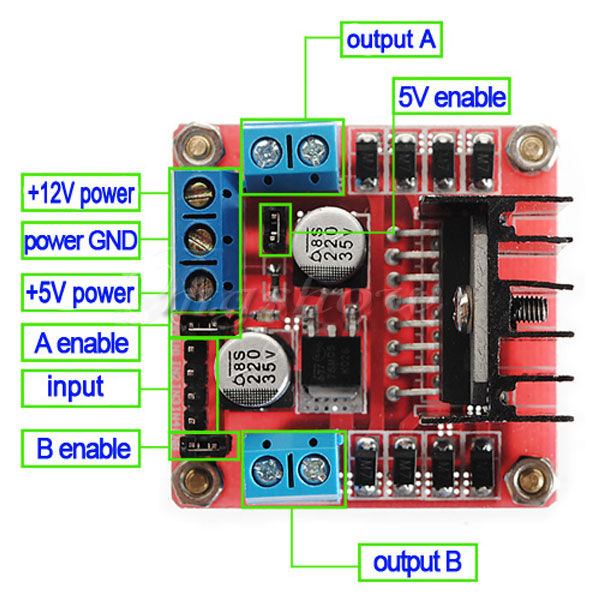
\includegraphics[scale=0.4]{Billeder/H-bro.jpg}
\caption{ En forudproduceret H-bro.}
\label{fig:mikrocontrollerprint}
\end{figure}

Til aftestning har gruppen gjort brug af en L289N-enhed. Dette er en færdig H-bro som bruges til at controllere retning og omdrejninger på en stepmotor/DC motor. Denne enhed har op til 6 input pins samt 1-2 pins til strømforsyning. Den ene af disse pins kan laves om til et output for en lav strømforsyning, for eksempel til en arduino, hvis der er forbundet en strømforsyning til den anden port på +12V. Den sidste pin skal forbindes til ground.

\subsection{Test af knapper}

Som en del af vores produkt har vi produceret en trådløs controller til at styre vores tårn med. denne controller fungere ved input gennem fem knapper, en til hver kommando. I vores forløb har vi prøvet flere forskellige opsætning af knapper, med hver deres modstand, en enkelt, og brug af forskellige ledninger. Det er blevet bestemt ud fra forsøg at et sådant knapsystem fungere bedst hvis alle knapper har deres egen modstand inden de går til jord, samt at mere ukonventionel opsætning og placering generelt skaber flere problemer end de løser. Ved brug af samme placering som på moderne spillemaskine-controller opstod der signalforstyrrelser som ikke var til at fjerne, og ved en enkelt stor modstand blev signalerne fra knapperne sjældent stoppet når de var blevet trykket ned.\\

I sidste ende har vi valgt at lave en række med fem knapper med hver deres modstand og en kombineret forbindelse til jord.

\subsection{Aftestning af mikrocontroller og mikrocontrollerprint}
Inden arbejdet med selve mikrocontrollerprintet begyndtes, testede vi kredsløbet på et fjumrebræt for at sikre, at det virkede som tiltænkt inden produktionen af printet startedes, da en fejl i printets design tager meget længere tid at fikse, hvis den opdages for sent.

\begin{figure}[H]
\centering
\includegraphics[scale=0.4]{Billeder/Fjumrebraet.jpg}
\caption{  Foerste test af mikrocontrollerprintet på et fjumrebraet. Oeverst til hoejre kan spaendingsregulatoren ses, mens ATMega’en og de tilhoerende forbindelser er til venstre.}
\label{fig:fjumrebraet}
\end{figure}

Efter at testen, som gik ud på at få en lysdiode til at stige og falde i lysstyrke, virkede på fjumrebrættet, kunne selve produktionen af mikrocontrollerprintet begynde. Da printet var blevet færdigproduceret testede vi alle forbindelser på det, for at opdage eventuelle produktionsfejl.

\begin{figure}[H]
\centering
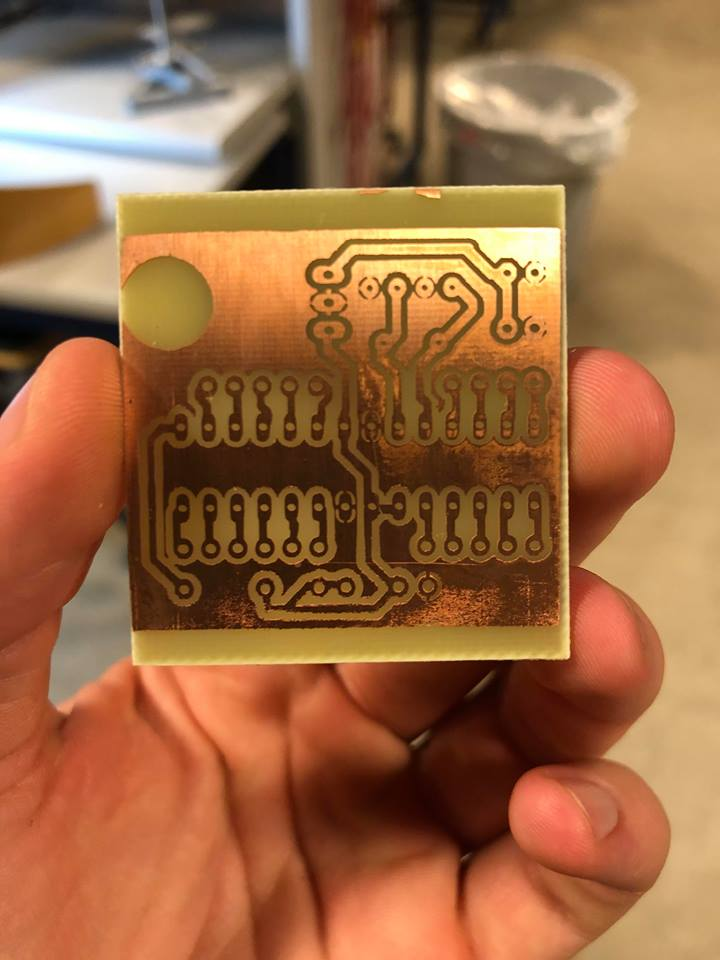
\includegraphics[scale=0.4]{Billeder/print.jpg}
\caption{ Kobberforbindelserne på det nylavede mikrocontrollerprint.}
\label{fig:print_test}
\end{figure}

Det første print vi lavede havde en fejl, da det var blevet spejlvendt under produktionen, hvilket gjorde at alle de “ikke-spejlbare” komponenter (ATMega328p og LM7805) skulle loddes fast på den modsatte side af printet, end hvor man normalt gør det. Der skulle altså loddes under selve komponenten istedet for på den anden side af printet. Det kom dog til at virke, selvom det var betydeligt mere vanskeligt loddearbejde end normalt.


\begin{figure}[H]
\centering
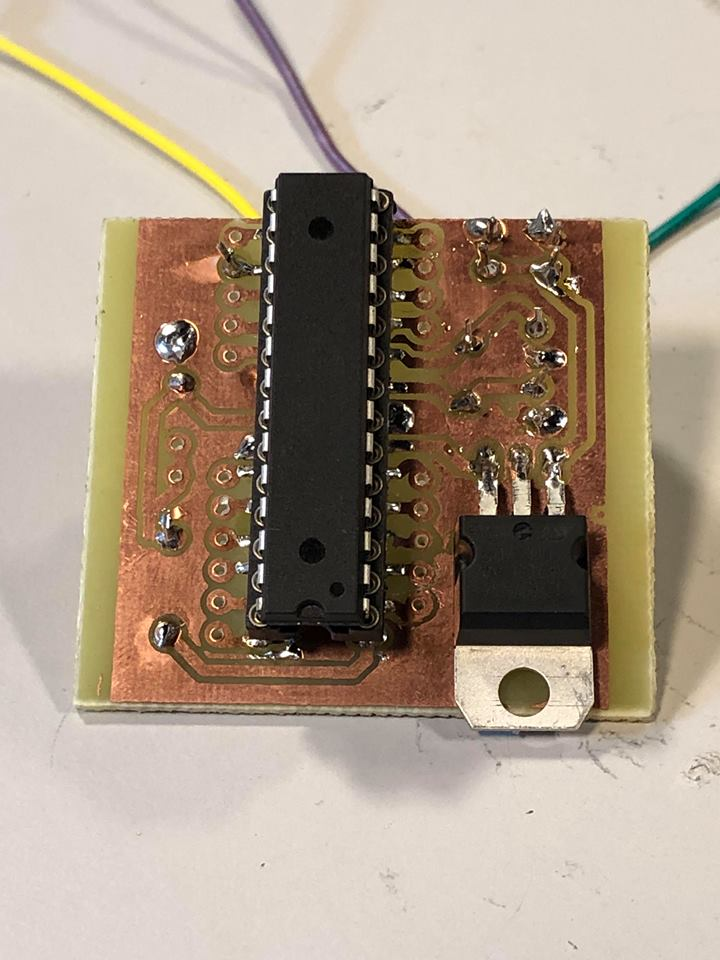
\includegraphics[scale=0.4]{Billeder/spejlvendtprint.jpg}
\caption{ Det færdiglavede og fuldt funktionelle spejlvendte print.}
\label{fig:print_test}
\end{figure}

Vi testede printets funktionalitet ved brug af den samme test, som før printarbejdet blev påbegyndt, da denne derfor var bevidst til at skulle virke. Vi lavede også et andet print, da vi ikke var sikre på om den spejlvendte kunne loddes korrekt, men denne havde flere produktionsfejl, da den manglede de anmærkede kobberbaner flere steder. Dette førte til, at den blev næsten umulig at lodde korrekt og skulle kasseres.

\begin{figure}[H]
\centering
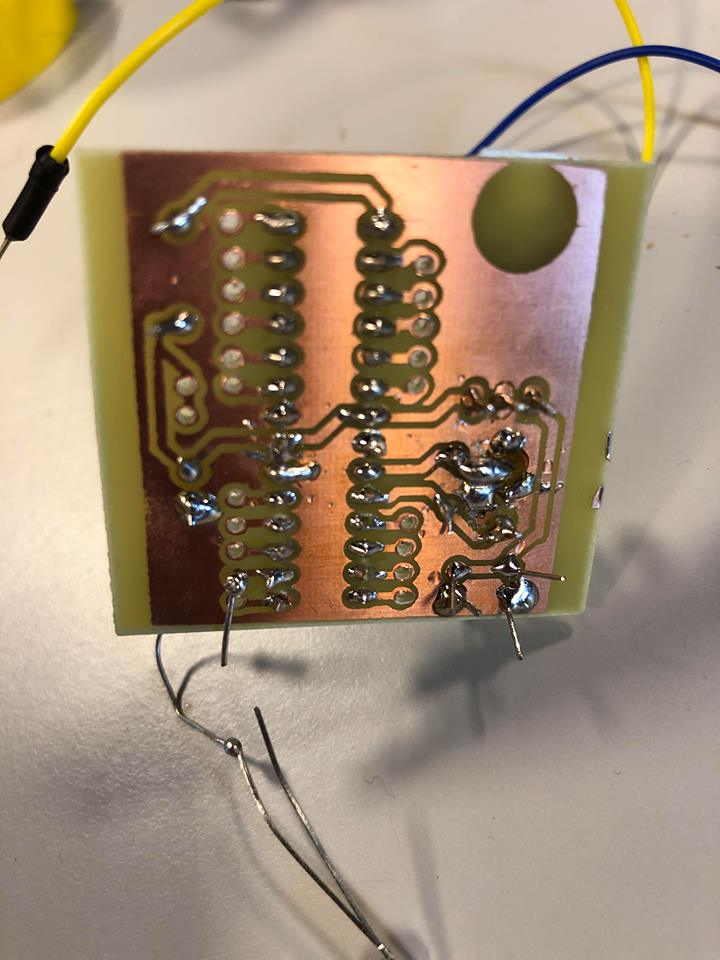
\includegraphics[scale=0.4]{Billeder/fejlprint.jpg}
\caption{ Loddefejlen nederst til hoejre på fejlprintet skyldes de manglende/beskadigede kobberbaner.}
\label{fig:print_test}
\end{figure}




\subsection{Problemer under udviklingen af produktet }
\subsubsection{Problem \#1 - Stepper motor vs. DC motor}
I den største del af projektet har vi i gruppen forsøgt at gøre brug af to stærke stepper motorer til at hæve og sænke geværet samt dreje selve platformen. Vi har dog haft store problemer med bare at få disse motorer til at lave simple rotationer. Det første problem vi stødte på var ikke at få selve motoren til at køre, det var at dem vi havde fundet var for svage og havde en for lav trækkraft. Disse blev så skiftet ud med to større motorer, som hver har en trækkraft på cirka 10 kg. Disse havde dog også et meget stort problem, de virkede kun halvdelen af tiden, den anden halvdel vibrerede de bare. Problemet opstod formentlig i enten koden eller selve kredsløbet, men begge disse er blevet ændret på alle tænkelige måder for at løse dette problem. I sidste ende har vi skiftet begge stepper motorer ud med DC motor, disse er både lettere at bruge, samt har de ingen af de samme problemer som stepper motorne havde. Der er dog et argument for at selve tårnets bevægelse ikke er lige så præcis, dog var selve ideen at den skulle dreje efter hvor længe man holder en bestemt knap inde, så selve den endelige bevægelse bliver ikke påvirket af dette skift af motoren.

\subsubsection{Problem \#2 - Flydende kommunikation}
I den sidste del af projektet har vi haft problemer med flydende bevægelser ud fra vores givne kommandoer, i et normalt program uden trådløs kommunikation ville man kunne opnå en “flydende overgang” fra kommando til handling ved at definere det ud fra et HIGH/LOW state, dette er dog ikke tilfældet her. Da man er nødt til at sende information som pakker er der ikke mulighed for at sende et kontinuerligt signal som kan ændre sig på samme måde som et HIGH/LOW state. For at skabe en flydende overgang skal den “pause” altså det delay, som er mellem hver kommando og udførelsen af en handling passe sammen, hvis der går længere tid mellem handlinger end mellem kommandoer ville dette resultere i at man ville kunne “indhente” den del af hardware som udføre handlingerne og endda overhale den, så den udføre handlinger, selvom man ikke trykker noget på det tidspunkt. Hvis man derimod har kortere mellem handlinger end mellem kommandoer ville det se ud som om at der er et “input lag” hvilket der i princippet også er. De to skal altså stemmer overens, man stadigt ikke ske så hurtigt at programmet og de mere mekaniske dele af hardware ikke kan følge med.\\

I disse to stykker kode ses de to tider som skal stemmer overens: 

\begin{lstlisting}[style=CStyle]
//Turret.ino

if(bluetooth.available()) //Hvis der er kommunikation med bluetooth, start switch
	switch ((char)bluetooth.read()){
		case 'a': //Hvis turret har modtaget char: a, drej til venstre i 250ms
			digitalWrite(R, LOW);
			digitalWrite(L, HIGH);
			digitalWrite(LodPin, statc);
			delay(250);
			serial.println("a");
			delay(1);
			break;	
			
\end{lstlisting}

\begin{lstlisting}[style=CStyle]
//Controller.ino

if(buttonStateLeft == HIGH){
	bluetooth.print((char) 'a');
	serial.println("a");
	delay(250);
}

\end{lstlisting}


I en længere periode var begge et helt sekund, dette resulterede i ringe kontrol og en fornemmelse af “lag” hvis man sænker tiden for handlingen uden at sænke for kommandoen vil der forekomme bevægelser i hak. 250 ms til hver lader til at være et sweet spot hvor der er en god følelse af kontrol, men også et punkt hvor motoren og H-broen kan nå at reagere på input fra Arduino.







